% Created by tikzDevice version 0.12.3.1 on 2022-04-28 16:22:14
% !TEX encoding = UTF-8 Unicode
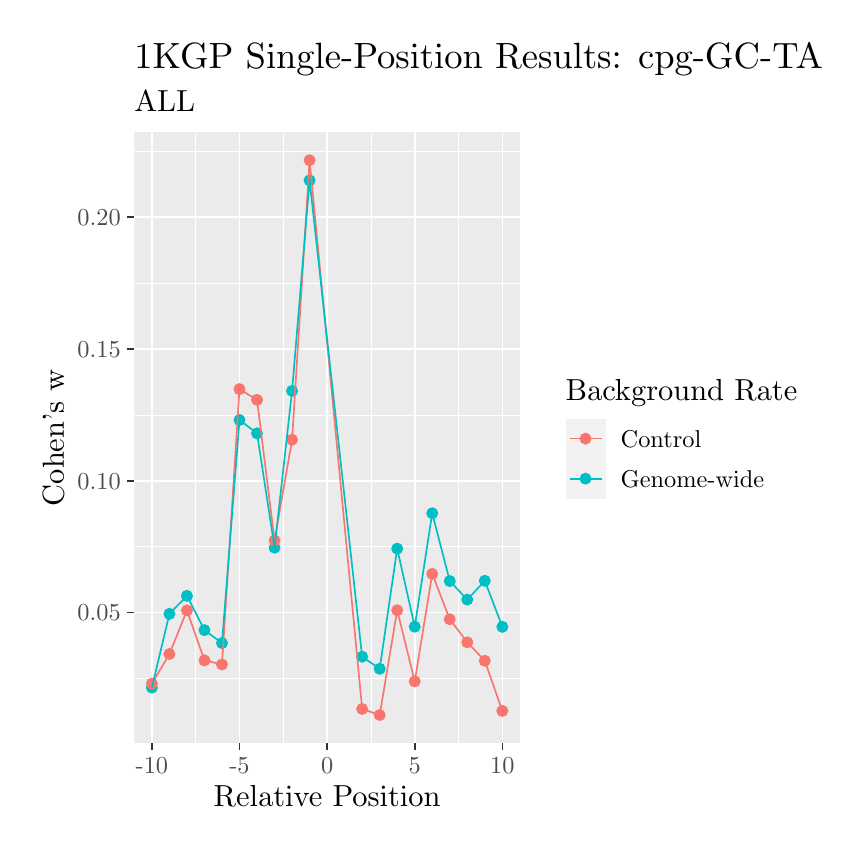
\begin{tikzpicture}[x=1pt,y=1pt]
\definecolor{fillColor}{RGB}{255,255,255}
\path[use as bounding box,fill=fillColor,fill opacity=0.00] (0,0) rectangle (289.08,289.08);
\begin{scope}
\path[clip] (  0.00,  0.00) rectangle (289.08,289.08);
\definecolor{drawColor}{RGB}{255,255,255}
\definecolor{fillColor}{RGB}{255,255,255}

\path[draw=drawColor,line width= 0.6pt,line join=round,line cap=round,fill=fillColor] (  0.00,  0.00) rectangle (289.08,289.08);
\end{scope}
\begin{scope}
\path[clip] ( 38.56, 30.69) rectangle (177.85,251.21);
\definecolor{fillColor}{gray}{0.92}

\path[fill=fillColor] ( 38.56, 30.69) rectangle (177.85,251.21);
\definecolor{drawColor}{RGB}{255,255,255}

\path[draw=drawColor,line width= 0.3pt,line join=round] ( 38.56, 53.91) --
	(177.85, 53.91);

\path[draw=drawColor,line width= 0.3pt,line join=round] ( 38.56,101.53) --
	(177.85,101.53);

\path[draw=drawColor,line width= 0.3pt,line join=round] ( 38.56,149.14) --
	(177.85,149.14);

\path[draw=drawColor,line width= 0.3pt,line join=round] ( 38.56,196.76) --
	(177.85,196.76);

\path[draw=drawColor,line width= 0.3pt,line join=round] ( 38.56,244.37) --
	(177.85,244.37);

\path[draw=drawColor,line width= 0.3pt,line join=round] ( 60.72, 30.69) --
	( 60.72,251.21);

\path[draw=drawColor,line width= 0.3pt,line join=round] ( 92.37, 30.69) --
	( 92.37,251.21);

\path[draw=drawColor,line width= 0.3pt,line join=round] (124.03, 30.69) --
	(124.03,251.21);

\path[draw=drawColor,line width= 0.3pt,line join=round] (155.69, 30.69) --
	(155.69,251.21);

\path[draw=drawColor,line width= 0.6pt,line join=round] ( 38.56, 77.72) --
	(177.85, 77.72);

\path[draw=drawColor,line width= 0.6pt,line join=round] ( 38.56,125.33) --
	(177.85,125.33);

\path[draw=drawColor,line width= 0.6pt,line join=round] ( 38.56,172.95) --
	(177.85,172.95);

\path[draw=drawColor,line width= 0.6pt,line join=round] ( 38.56,220.57) --
	(177.85,220.57);

\path[draw=drawColor,line width= 0.6pt,line join=round] ( 44.89, 30.69) --
	( 44.89,251.21);

\path[draw=drawColor,line width= 0.6pt,line join=round] ( 76.54, 30.69) --
	( 76.54,251.21);

\path[draw=drawColor,line width= 0.6pt,line join=round] (108.20, 30.69) --
	(108.20,251.21);

\path[draw=drawColor,line width= 0.6pt,line join=round] (139.86, 30.69) --
	(139.86,251.21);

\path[draw=drawColor,line width= 0.6pt,line join=round] (171.52, 30.69) --
	(171.52,251.21);
\definecolor{drawColor}{RGB}{0,191,196}
\definecolor{fillColor}{RGB}{0,191,196}

\path[draw=drawColor,line width= 0.4pt,line join=round,line cap=round,fill=fillColor] ( 44.89, 50.61) circle (  1.96);
\definecolor{drawColor}{RGB}{248,118,109}
\definecolor{fillColor}{RGB}{248,118,109}

\path[draw=drawColor,line width= 0.4pt,line join=round,line cap=round,fill=fillColor] ( 44.89, 52.04) circle (  1.96);
\definecolor{drawColor}{RGB}{0,191,196}
\definecolor{fillColor}{RGB}{0,191,196}

\path[draw=drawColor,line width= 0.4pt,line join=round,line cap=round,fill=fillColor] ( 51.22, 77.26) circle (  1.96);
\definecolor{drawColor}{RGB}{248,118,109}
\definecolor{fillColor}{RGB}{248,118,109}

\path[draw=drawColor,line width= 0.4pt,line join=round,line cap=round,fill=fillColor] ( 51.22, 62.76) circle (  1.96);
\definecolor{drawColor}{RGB}{0,191,196}
\definecolor{fillColor}{RGB}{0,191,196}

\path[draw=drawColor,line width= 0.4pt,line join=round,line cap=round,fill=fillColor] ( 57.55, 83.77) circle (  1.96);
\definecolor{drawColor}{RGB}{248,118,109}
\definecolor{fillColor}{RGB}{248,118,109}

\path[draw=drawColor,line width= 0.4pt,line join=round,line cap=round,fill=fillColor] ( 57.55, 78.50) circle (  1.96);
\definecolor{drawColor}{RGB}{0,191,196}
\definecolor{fillColor}{RGB}{0,191,196}

\path[draw=drawColor,line width= 0.4pt,line join=round,line cap=round,fill=fillColor] ( 63.88, 71.39) circle (  1.96);
\definecolor{drawColor}{RGB}{248,118,109}
\definecolor{fillColor}{RGB}{248,118,109}

\path[draw=drawColor,line width= 0.4pt,line join=round,line cap=round,fill=fillColor] ( 63.88, 60.45) circle (  1.96);
\definecolor{drawColor}{RGB}{0,191,196}
\definecolor{fillColor}{RGB}{0,191,196}

\path[draw=drawColor,line width= 0.4pt,line join=round,line cap=round,fill=fillColor] ( 70.21, 66.71) circle (  1.96);
\definecolor{drawColor}{RGB}{248,118,109}
\definecolor{fillColor}{RGB}{248,118,109}

\path[draw=drawColor,line width= 0.4pt,line join=round,line cap=round,fill=fillColor] ( 70.21, 58.99) circle (  1.96);
\definecolor{drawColor}{RGB}{0,191,196}
\definecolor{fillColor}{RGB}{0,191,196}

\path[draw=drawColor,line width= 0.4pt,line join=round,line cap=round,fill=fillColor] ( 76.54,147.32) circle (  1.96);
\definecolor{drawColor}{RGB}{248,118,109}
\definecolor{fillColor}{RGB}{248,118,109}

\path[draw=drawColor,line width= 0.4pt,line join=round,line cap=round,fill=fillColor] ( 76.54,158.46) circle (  1.96);
\definecolor{drawColor}{RGB}{0,191,196}
\definecolor{fillColor}{RGB}{0,191,196}

\path[draw=drawColor,line width= 0.4pt,line join=round,line cap=round,fill=fillColor] ( 82.88,142.50) circle (  1.96);
\definecolor{drawColor}{RGB}{248,118,109}
\definecolor{fillColor}{RGB}{248,118,109}

\path[draw=drawColor,line width= 0.4pt,line join=round,line cap=round,fill=fillColor] ( 82.88,154.59) circle (  1.96);
\definecolor{drawColor}{RGB}{0,191,196}
\definecolor{fillColor}{RGB}{0,191,196}

\path[draw=drawColor,line width= 0.4pt,line join=round,line cap=round,fill=fillColor] ( 89.21,101.17) circle (  1.96);
\definecolor{drawColor}{RGB}{248,118,109}
\definecolor{fillColor}{RGB}{248,118,109}

\path[draw=drawColor,line width= 0.4pt,line join=round,line cap=round,fill=fillColor] ( 89.21,103.78) circle (  1.96);
\definecolor{drawColor}{RGB}{0,191,196}
\definecolor{fillColor}{RGB}{0,191,196}

\path[draw=drawColor,line width= 0.4pt,line join=round,line cap=round,fill=fillColor] ( 95.54,157.83) circle (  1.96);
\definecolor{drawColor}{RGB}{248,118,109}
\definecolor{fillColor}{RGB}{248,118,109}

\path[draw=drawColor,line width= 0.4pt,line join=round,line cap=round,fill=fillColor] ( 95.54,140.19) circle (  1.96);
\definecolor{drawColor}{RGB}{0,191,196}
\definecolor{fillColor}{RGB}{0,191,196}

\path[draw=drawColor,line width= 0.4pt,line join=round,line cap=round,fill=fillColor] (101.87,233.90) circle (  1.96);
\definecolor{drawColor}{RGB}{248,118,109}
\definecolor{fillColor}{RGB}{248,118,109}

\path[draw=drawColor,line width= 0.4pt,line join=round,line cap=round,fill=fillColor] (101.87,241.18) circle (  1.96);
\definecolor{drawColor}{RGB}{0,191,196}
\definecolor{fillColor}{RGB}{0,191,196}

\path[draw=drawColor,line width= 0.4pt,line join=round,line cap=round,fill=fillColor] (120.86, 61.78) circle (  1.96);
\definecolor{drawColor}{RGB}{248,118,109}
\definecolor{fillColor}{RGB}{248,118,109}

\path[draw=drawColor,line width= 0.4pt,line join=round,line cap=round,fill=fillColor] (120.86, 42.89) circle (  1.96);
\definecolor{drawColor}{RGB}{0,191,196}
\definecolor{fillColor}{RGB}{0,191,196}

\path[draw=drawColor,line width= 0.4pt,line join=round,line cap=round,fill=fillColor] (127.20, 57.40) circle (  1.96);
\definecolor{drawColor}{RGB}{248,118,109}
\definecolor{fillColor}{RGB}{248,118,109}

\path[draw=drawColor,line width= 0.4pt,line join=round,line cap=round,fill=fillColor] (127.20, 40.71) circle (  1.96);
\definecolor{drawColor}{RGB}{0,191,196}
\definecolor{fillColor}{RGB}{0,191,196}

\path[draw=drawColor,line width= 0.4pt,line join=round,line cap=round,fill=fillColor] (133.53,100.82) circle (  1.96);
\definecolor{drawColor}{RGB}{248,118,109}
\definecolor{fillColor}{RGB}{248,118,109}

\path[draw=drawColor,line width= 0.4pt,line join=round,line cap=round,fill=fillColor] (133.53, 78.55) circle (  1.96);
\definecolor{drawColor}{RGB}{0,191,196}
\definecolor{fillColor}{RGB}{0,191,196}

\path[draw=drawColor,line width= 0.4pt,line join=round,line cap=round,fill=fillColor] (139.86, 72.63) circle (  1.96);
\definecolor{drawColor}{RGB}{248,118,109}
\definecolor{fillColor}{RGB}{248,118,109}

\path[draw=drawColor,line width= 0.4pt,line join=round,line cap=round,fill=fillColor] (139.86, 52.87) circle (  1.96);
\definecolor{drawColor}{RGB}{0,191,196}
\definecolor{fillColor}{RGB}{0,191,196}

\path[draw=drawColor,line width= 0.4pt,line join=round,line cap=round,fill=fillColor] (146.19,113.62) circle (  1.96);
\definecolor{drawColor}{RGB}{248,118,109}
\definecolor{fillColor}{RGB}{248,118,109}

\path[draw=drawColor,line width= 0.4pt,line join=round,line cap=round,fill=fillColor] (146.19, 91.71) circle (  1.96);
\definecolor{drawColor}{RGB}{0,191,196}
\definecolor{fillColor}{RGB}{0,191,196}

\path[draw=drawColor,line width= 0.4pt,line join=round,line cap=round,fill=fillColor] (152.52, 89.11) circle (  1.96);
\definecolor{drawColor}{RGB}{248,118,109}
\definecolor{fillColor}{RGB}{248,118,109}

\path[draw=drawColor,line width= 0.4pt,line join=round,line cap=round,fill=fillColor] (152.52, 75.31) circle (  1.96);
\definecolor{drawColor}{RGB}{0,191,196}
\definecolor{fillColor}{RGB}{0,191,196}

\path[draw=drawColor,line width= 0.4pt,line join=round,line cap=round,fill=fillColor] (158.85, 82.42) circle (  1.96);
\definecolor{drawColor}{RGB}{248,118,109}
\definecolor{fillColor}{RGB}{248,118,109}

\path[draw=drawColor,line width= 0.4pt,line join=round,line cap=round,fill=fillColor] (158.85, 66.98) circle (  1.96);
\definecolor{drawColor}{RGB}{0,191,196}
\definecolor{fillColor}{RGB}{0,191,196}

\path[draw=drawColor,line width= 0.4pt,line join=round,line cap=round,fill=fillColor] (165.18, 89.20) circle (  1.96);
\definecolor{drawColor}{RGB}{248,118,109}
\definecolor{fillColor}{RGB}{248,118,109}

\path[draw=drawColor,line width= 0.4pt,line join=round,line cap=round,fill=fillColor] (165.18, 60.31) circle (  1.96);
\definecolor{drawColor}{RGB}{0,191,196}
\definecolor{fillColor}{RGB}{0,191,196}

\path[draw=drawColor,line width= 0.4pt,line join=round,line cap=round,fill=fillColor] (171.52, 72.57) circle (  1.96);
\definecolor{drawColor}{RGB}{248,118,109}
\definecolor{fillColor}{RGB}{248,118,109}

\path[draw=drawColor,line width= 0.4pt,line join=round,line cap=round,fill=fillColor] (171.52, 42.19) circle (  1.96);

\path[draw=drawColor,line width= 0.6pt,line join=round] ( 44.89, 52.04) --
	( 51.22, 62.76) --
	( 57.55, 78.50) --
	( 63.88, 60.45) --
	( 70.21, 58.99) --
	( 76.54,158.46) --
	( 82.88,154.59) --
	( 89.21,103.78) --
	( 95.54,140.19) --
	(101.87,241.18) --
	(120.86, 42.89) --
	(127.20, 40.71) --
	(133.53, 78.55) --
	(139.86, 52.87) --
	(146.19, 91.71) --
	(152.52, 75.31) --
	(158.85, 66.98) --
	(165.18, 60.31) --
	(171.52, 42.19);
\definecolor{drawColor}{RGB}{0,191,196}

\path[draw=drawColor,line width= 0.6pt,line join=round] ( 44.89, 50.61) --
	( 51.22, 77.26) --
	( 57.55, 83.77) --
	( 63.88, 71.39) --
	( 70.21, 66.71) --
	( 76.54,147.32) --
	( 82.88,142.50) --
	( 89.21,101.17) --
	( 95.54,157.83) --
	(101.87,233.90) --
	(120.86, 61.78) --
	(127.20, 57.40) --
	(133.53,100.82) --
	(139.86, 72.63) --
	(146.19,113.62) --
	(152.52, 89.11) --
	(158.85, 82.42) --
	(165.18, 89.20) --
	(171.52, 72.57);
\end{scope}
\begin{scope}
\path[clip] (  0.00,  0.00) rectangle (289.08,289.08);
\definecolor{drawColor}{gray}{0.30}

\node[text=drawColor,anchor=base east,inner sep=0pt, outer sep=0pt, scale=  0.88] at ( 33.61, 74.69) {0.05};

\node[text=drawColor,anchor=base east,inner sep=0pt, outer sep=0pt, scale=  0.88] at ( 33.61,122.30) {0.10};

\node[text=drawColor,anchor=base east,inner sep=0pt, outer sep=0pt, scale=  0.88] at ( 33.61,169.92) {0.15};

\node[text=drawColor,anchor=base east,inner sep=0pt, outer sep=0pt, scale=  0.88] at ( 33.61,217.53) {0.20};
\end{scope}
\begin{scope}
\path[clip] (  0.00,  0.00) rectangle (289.08,289.08);
\definecolor{drawColor}{gray}{0.20}

\path[draw=drawColor,line width= 0.6pt,line join=round] ( 35.81, 77.72) --
	( 38.56, 77.72);

\path[draw=drawColor,line width= 0.6pt,line join=round] ( 35.81,125.33) --
	( 38.56,125.33);

\path[draw=drawColor,line width= 0.6pt,line join=round] ( 35.81,172.95) --
	( 38.56,172.95);

\path[draw=drawColor,line width= 0.6pt,line join=round] ( 35.81,220.57) --
	( 38.56,220.57);
\end{scope}
\begin{scope}
\path[clip] (  0.00,  0.00) rectangle (289.08,289.08);
\definecolor{drawColor}{gray}{0.20}

\path[draw=drawColor,line width= 0.6pt,line join=round] ( 44.89, 27.94) --
	( 44.89, 30.69);

\path[draw=drawColor,line width= 0.6pt,line join=round] ( 76.54, 27.94) --
	( 76.54, 30.69);

\path[draw=drawColor,line width= 0.6pt,line join=round] (108.20, 27.94) --
	(108.20, 30.69);

\path[draw=drawColor,line width= 0.6pt,line join=round] (139.86, 27.94) --
	(139.86, 30.69);

\path[draw=drawColor,line width= 0.6pt,line join=round] (171.52, 27.94) --
	(171.52, 30.69);
\end{scope}
\begin{scope}
\path[clip] (  0.00,  0.00) rectangle (289.08,289.08);
\definecolor{drawColor}{gray}{0.30}

\node[text=drawColor,anchor=base,inner sep=0pt, outer sep=0pt, scale=  0.88] at ( 44.89, 19.68) {-10};

\node[text=drawColor,anchor=base,inner sep=0pt, outer sep=0pt, scale=  0.88] at ( 76.54, 19.68) {-5};

\node[text=drawColor,anchor=base,inner sep=0pt, outer sep=0pt, scale=  0.88] at (108.20, 19.68) {0};

\node[text=drawColor,anchor=base,inner sep=0pt, outer sep=0pt, scale=  0.88] at (139.86, 19.68) {5};

\node[text=drawColor,anchor=base,inner sep=0pt, outer sep=0pt, scale=  0.88] at (171.52, 19.68) {10};
\end{scope}
\begin{scope}
\path[clip] (  0.00,  0.00) rectangle (289.08,289.08);
\definecolor{drawColor}{RGB}{0,0,0}

\node[text=drawColor,anchor=base,inner sep=0pt, outer sep=0pt, scale=  1.10] at (108.20,  7.64) {Relative Position};
\end{scope}
\begin{scope}
\path[clip] (  0.00,  0.00) rectangle (289.08,289.08);
\definecolor{drawColor}{RGB}{0,0,0}

\node[text=drawColor,rotate= 90.00,anchor=base,inner sep=0pt, outer sep=0pt, scale=  1.10] at ( 13.08,140.95) {Cohen's w};
\end{scope}
\begin{scope}
\path[clip] (  0.00,  0.00) rectangle (289.08,289.08);
\definecolor{fillColor}{RGB}{255,255,255}

\path[fill=fillColor] (188.85,113.39) rectangle (283.58,168.51);
\end{scope}
\begin{scope}
\path[clip] (  0.00,  0.00) rectangle (289.08,289.08);
\definecolor{drawColor}{RGB}{0,0,0}

\node[text=drawColor,anchor=base west,inner sep=0pt, outer sep=0pt, scale=  1.10] at (194.35,154.36) {Background Rate};
\end{scope}
\begin{scope}
\path[clip] (  0.00,  0.00) rectangle (289.08,289.08);
\definecolor{fillColor}{gray}{0.95}

\path[fill=fillColor] (194.35,133.34) rectangle (208.80,147.79);
\end{scope}
\begin{scope}
\path[clip] (  0.00,  0.00) rectangle (289.08,289.08);
\definecolor{drawColor}{RGB}{248,118,109}
\definecolor{fillColor}{RGB}{248,118,109}

\path[draw=drawColor,line width= 0.4pt,line join=round,line cap=round,fill=fillColor] (201.57,140.57) circle (  1.96);
\end{scope}
\begin{scope}
\path[clip] (  0.00,  0.00) rectangle (289.08,289.08);
\definecolor{drawColor}{RGB}{248,118,109}

\path[draw=drawColor,line width= 0.6pt,line join=round] (195.79,140.57) -- (207.36,140.57);
\end{scope}
\begin{scope}
\path[clip] (  0.00,  0.00) rectangle (289.08,289.08);
\definecolor{fillColor}{gray}{0.95}

\path[fill=fillColor] (194.35,118.89) rectangle (208.80,133.34);
\end{scope}
\begin{scope}
\path[clip] (  0.00,  0.00) rectangle (289.08,289.08);
\definecolor{drawColor}{RGB}{0,191,196}
\definecolor{fillColor}{RGB}{0,191,196}

\path[draw=drawColor,line width= 0.4pt,line join=round,line cap=round,fill=fillColor] (201.57,126.11) circle (  1.96);
\end{scope}
\begin{scope}
\path[clip] (  0.00,  0.00) rectangle (289.08,289.08);
\definecolor{drawColor}{RGB}{0,191,196}

\path[draw=drawColor,line width= 0.6pt,line join=round] (195.79,126.11) -- (207.36,126.11);
\end{scope}
\begin{scope}
\path[clip] (  0.00,  0.00) rectangle (289.08,289.08);
\definecolor{drawColor}{RGB}{0,0,0}

\node[text=drawColor,anchor=base west,inner sep=0pt, outer sep=0pt, scale=  0.88] at (214.30,137.54) {Control};
\end{scope}
\begin{scope}
\path[clip] (  0.00,  0.00) rectangle (289.08,289.08);
\definecolor{drawColor}{RGB}{0,0,0}

\node[text=drawColor,anchor=base west,inner sep=0pt, outer sep=0pt, scale=  0.88] at (214.30,123.08) {Genome-wide};
\end{scope}
\begin{scope}
\path[clip] (  0.00,  0.00) rectangle (289.08,289.08);
\definecolor{drawColor}{RGB}{0,0,0}

\node[text=drawColor,anchor=base west,inner sep=0pt, outer sep=0pt, scale=  1.10] at ( 38.56,258.85) {ALL};
\end{scope}
\begin{scope}
\path[clip] (  0.00,  0.00) rectangle (289.08,289.08);
\definecolor{drawColor}{RGB}{0,0,0}

\node[text=drawColor,anchor=base west,inner sep=0pt, outer sep=0pt, scale=  1.32] at ( 38.56,274.49) {1KGP Single-Position Results: cpg-GC-TA};
\end{scope}
\end{tikzpicture}
